\documentclass{article}[18pt]
\usepackage[utf8]{inputenc}
\usepackage[margin=0.7in]{geometry}
\usepackage{parselines} 
\usepackage{amsmath}
\usepackage{titlesec}
\usepackage{pgfplots}
\usepackage{graphicx}
\usepackage{tabularx}
\usepackage[english]{babel}
\usepackage{fancyhdr}
\usepackage{circuitikz}
\usetikzlibrary{decorations.pathmorphing,arrows}

\pgfplotsset{width=10cm,compat=1.9}
\usepackage{relsize}
\titlespacing\section{0pt}{14pt plus 4pt minus 2pt}{0pt plus 2pt minus 2pt}
\newlength\tindent
\setlength{\tindent}{\parindent}
\setlength{\parindent}{0pt}
\renewcommand{\indent}{\hspace*{\tindent}}

\pagestyle{fancy}
\fancyhf{}
\rhead{Sam Robbins 13SE}
\lhead{AS Level Physics - Waves}
\rfoot{Page \thepage}

\pgfkeys{/pgfplots/Axis Style/.style={
    width=13.5cm, height=10cm,
    axis x line=center, 
    axis y line=middle, 
    samples=100,
    ymin=-1.2, ymax=1.2,
    xmin=0, xmax=13.0,
    domain=-4*pi:4*pi
}}
\pgfkeys{/pgfplots/Stationary Wave/.style={
    width=13.5cm, height=5cm,
    axis x line=center, 
    axis y line=middle, 
    samples=100,
    ymin=-1.2, ymax=1.2,
    xmin=0, xmax=13.0,
    domain=-4*pi:4*pi
}}

\begin{document}
\begin{center}
\underline{\huge Progressive and stationary waves}
\end{center}
\section{Progressive waves}
\subsection{Transverse wave}
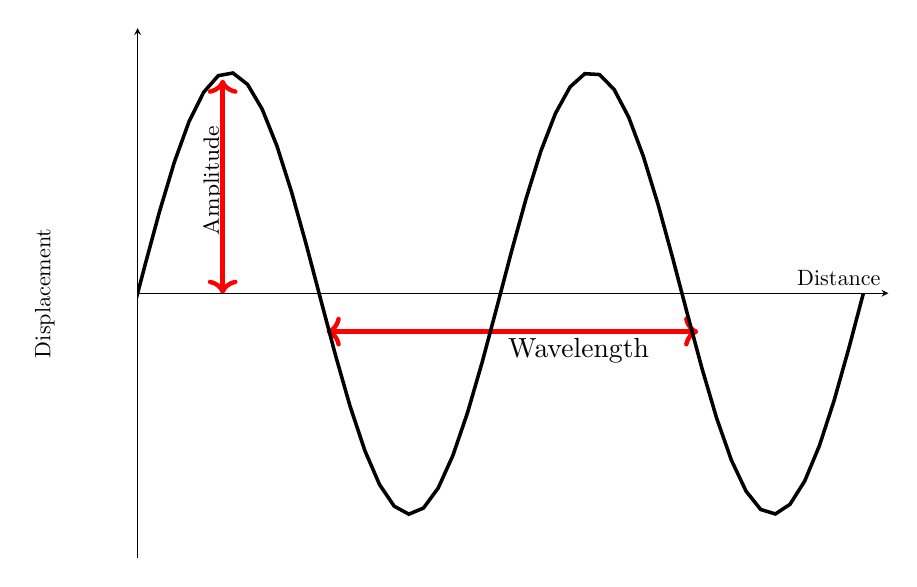
\begin{tikzpicture}[scale=0.8]
\tikzstyle{vlabel} = [fill=white,font=\footnotesize,inner sep=1pt,rotate=90]
\tikzstyle{hlabel} = [fill=white,font=\normalsize,inner sep=1pt]
\node[vlabel] at (1.2,6) {Amplitude};
\draw[arrows=<->,red,ultra thick](1.35,4.2)--(1.35,7.6);
\node[hlabel] at (7,3.3) {Wavelength};
\draw[arrows=<->,red,ultra thick](3,3.6)--(8.9,3.6);

\begin{axis}[
    Axis Style,
    y label style={at={(axis description cs:-0.1,.5)},rotate=90,anchor=south},
    ylabel = {Displacement},
    xlabel= {Distance},
    ticks=none
]
\addplot [mark=none, ultra thick, black] {sin(deg(x))};
\end{axis}
\end{tikzpicture}
\\
\\
Wave direction and energy are perpendicular
\subsection{Longitudinal wave}
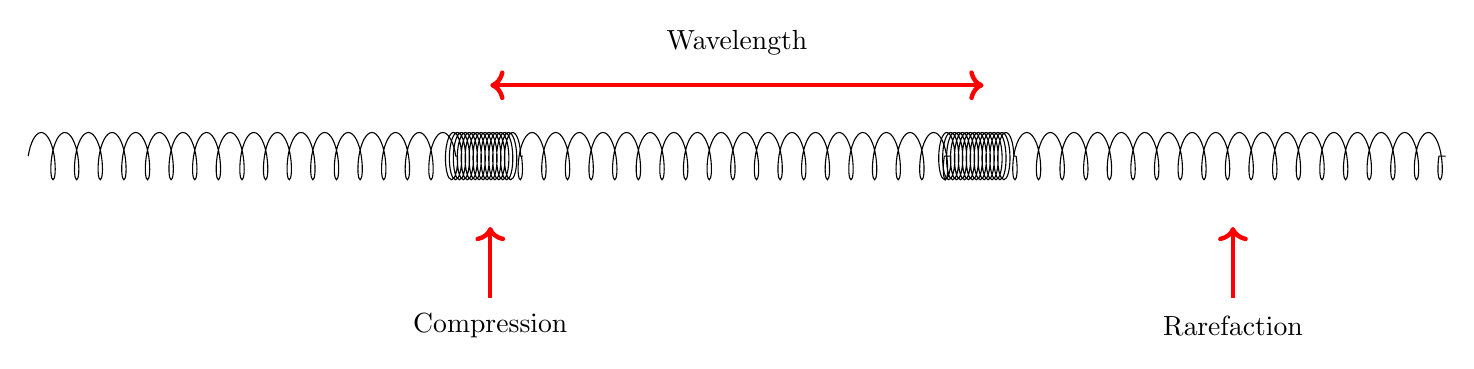
\begin{tikzpicture}[decoration={coil},scale=1.8]
\tikzstyle{hlabel} = [fill=white,font=\normalsize,inner sep=1pt]
\node[hlabel] at (5,0.8) {Wavelength};

\draw[arrows=<->,red,ultra thick](3.26,0.5)--(6.74,0.5);
\draw[arrows=->,red,ultra thick](3.26,-1)--(3.26,-0.5);
\draw[arrows=->,red,ultra thick](8.5,-1)--(8.5,-0.5);
\node[hlabel] at (3.26,-1.2) {Compression};
\node[hlabel] at (8.5,-1.2) {Rarefaction};
\draw[decorate, decoration={aspect=0.3, segment length=3mm, amplitude=3mm}] (0,0) --(3.03,0);
\draw[decorate, decoration={aspect=0.3, segment length=0.5mm, amplitude=-3mm}] (3.03,0) -- (3.49,0); 
\draw[decorate, decoration={aspect=0.3, segment length=3mm, amplitude=-3mm}] (3.48,0) -- (6.51,0);
\draw[decorate, decoration={aspect=0.3, segment length=0.5mm, amplitude=-3mm}] (6.51,0) -- (6.97,0);
\draw[decorate, decoration={aspect=0.3, segment length=3mm, amplitude=-3mm}] (6.97,0) -- (10,0);
\end{tikzpicture}
\\
\\
<<<<<<< HEAD
Wave direction and energy are parallel
=======
wave direction and energy are parallel
>>>>>>> master
\subsection{Definitions}
\textbf{Displacement} - Distance from equilibrium  to the position of the particle\\
\textbf{Amplitude} - The maximum displacement of a particle\\
\textbf{Wavelength} - The distance from a point on a wave to the same point on the next wave\\
\textbf{Complete cycle} - The cycle from one point of maximum displacement to the next section of maximum displacement\\
\textbf{Period} - The time for 1 complete cycle\\
\textbf{Frequency} - The number of complete cycles per second
\newpage
\subsection{Polarisation}
Polarised light all travels in the same direction\\
Unpolarised light travels in all directions\\
Unpolarised light can be polarised using a polarising filter which contains stripes, only allowing one direction of light through\\
\textbf{Only transverse waves can be polarised}
\\
\\
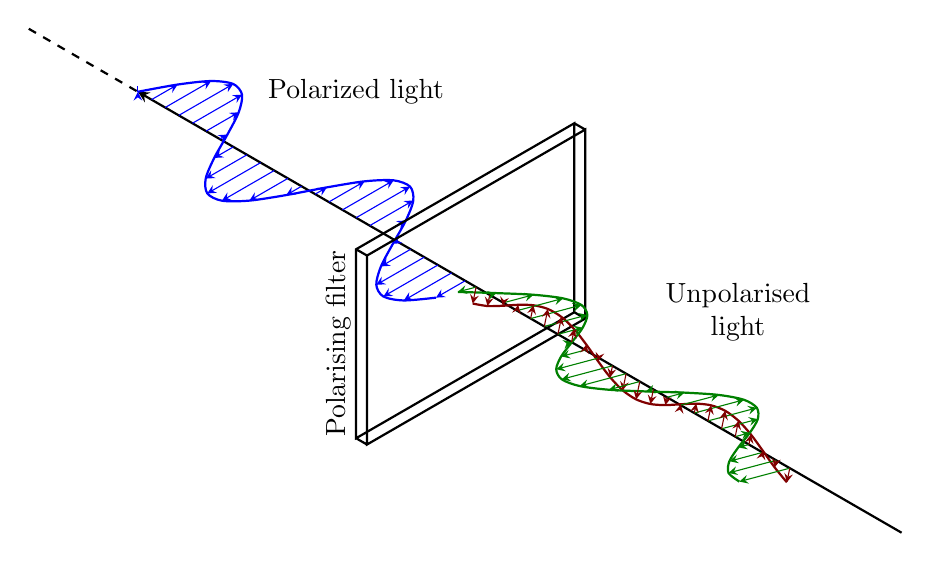
\begin{tikzpicture}[x={(0.866cm,-0.5cm)}, y={(0.866cm,0.5cm)}, z={(0cm,1cm)}, scale=.8,
    %Option for nice arrows
    >=stealth, %
    inner sep=0pt, outer sep=2pt,%
    axis/.style={thick,<-},
    wave/.style={thick,color=#1,smooth},
    polaroid/.style={fill=black!60!white, opacity=0.3},
]
    % Colors
    \colorlet{darkgreen}{green!50!black}
    \colorlet{lightgreen}{green!80!black}
    \colorlet{darkred}{red!50!black}
    \colorlet{lightred}{red!80!black}

    % Frame
    \coordinate (O) at (0, 0, 0);
    \draw[axis] (O) -- +(14, 0,   0);
    \draw[thick,dashed] (-2,0,0) -- (0,0,0);

    % Electric field vectors
    \draw[wave=blue, variable=\x,samples at={0,0.25,...,6}]
        plot (\x,{sin(2*\x r)},0);
    %Polarized light between polaroid and thin section
    \foreach \x in{0, 0.25,...,6}
        \draw[color=blue,->] (\x,0,0) -- (\x,{sin(2*\x r)},0);

    \draw (3,1,1) node [text width=2.5cm, text centered]{Polarized light};

    %Crystal thin section
    \begin{scope}[thick]
        \draw (6,-2,-1.5) -- (6,-2,1.5) node [above, sloped, midway]{Polarising filter}
                -- (6, 2, 1.5) -- (6, 2, -1.5) -- cycle % First face
            (6,  -2, -1.5) -- (6.2, -2,-1.5)
            (6,   2, -1.5) -- (6.2,  2,-1.5)
            (6,  -2,  1.5) -- (6.2, -2, 1.5)
            (6,   2,  1.5) -- (6.2,  2, 1.5)
            (6.2,-2, -1.5) -- (6.2, -2, 1.5) -- (6.2, 2, 1.5) 
                -- (6.2, 2, -1.5) -- cycle; % Second face
    \end{scope}

    %Rays leaving thin section
    \draw[wave=darkred,   variable=\x, samples at={6.2,6.45,...,12}] 
        plot (\x, {0.26*0.26*sin(2*(\x-0.5) r)},  {0.966*0.26*sin(2*(\x-0.5) r)});  %n'g-oriented ray
    \draw[wave=darkgreen, variable=\x, samples at={6.2,6.45,...,12}]
        plot (\x, {0.966*0.966*sin(2*(\x-0.1) r)},{-0.26*0.966*sin(2*(\x-0.1) r)}); %n'p-oriented ray
    \draw (10,1,1) node [text width=2.5cm, text centered] {Unpolarised light};

    \foreach \x in{6.2,6.45,...,12} {
        \draw[color=darkgreen, ->] (\x, 0, 0) --
            (\x, {0.966*0.966*sin(2*(\x-0.1) r)}, {-0.26*0.966*sin(2*(\x-0.1) r)});
        \draw[color=darkred,   ->] (\x, 0, 0) --
            (\x, {0.26*0.26*sin(2*(\x-0.5) r)}, {0.966*0.26*sin(2*(\x-0.5) r)});
            }
\end{tikzpicture}
\section{The superposition of waves and stationary waves}
Stationary waves are formed when a wave collides with itself after reflection\\
\\
\\
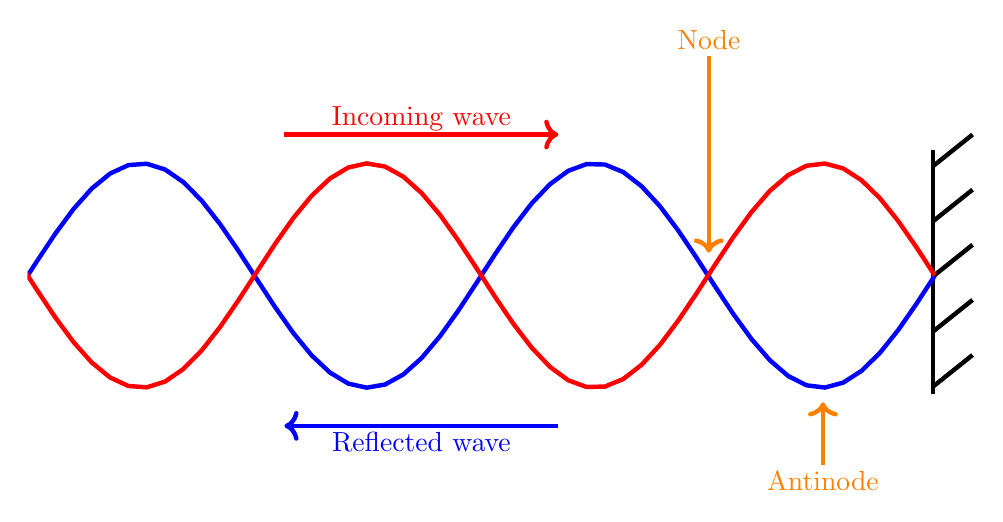
\begin{tikzpicture}
\draw[black,ultra thick] (11.5,0.2) -- ++(0,3.1);
\draw[black,ultra thick] (11.5,0.3) -- (12,0.7);
\draw[black,ultra thick] (11.5,1) -- ++(0.5,0.4);
\draw[black,ultra thick] (11.5,1.7) -- ++(0.5,0.4);
\draw[black,ultra thick] (11.5,2.4) -- ++(0.5,0.4);
\draw[black,ultra thick] (11.5,3.1) -- ++(0.5,0.4);
\tikzstyle{hlabel} = [font=\normalsize,inner sep=1pt]
\draw[arrows=->,red,ultra thick](3.26,3.5)--(6.74,3.5);
\node[hlabel,red] at (5,3.7) {Incoming wave};
\draw[arrows=<-,blue,ultra thick](3.26,-0.2)--(6.74,-0.2);
\node[hlabel,blue] at (5,-0.4) {Reflected wave};
\draw[arrows=->,orange,ultra thick](10.1,-0.7)-- ++(0,0.8);
\node[hlabel,orange] at (10.1,-0.9) {Antinode};

\draw[arrows=->,orange,ultra thick](8.65,4.5)-- ++(0,-2.5);
\node[hlabel,orange] at (8.65,4.7) {Node};



\begin{axis}[
    Stationary Wave,
    ticks=none,
    axis line style={draw=none}
]
\addplot [mark=none, ultra thick, blue] {sin(deg(x))};
\addplot [mark=none, ultra thick, red] {sin(deg(x+pi))};
\end{axis}
\end{tikzpicture}
\\
When both waves are at equilibrium there is a \textbf{node}\\
When one wave is at a maximum and one at a minimum there is an \textbf{antinode}\\
\subsection{Sound}
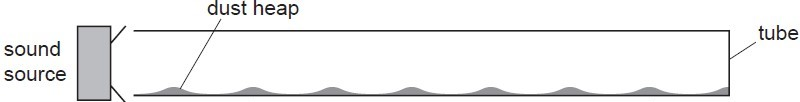
\includegraphics[width=15cm]{Sound.jpg}\\
Dust heaps are made at nodes and dips are made at antinodes\\
$\lambda$=Distance between the nodes $\times2$
\subsection{Microwaves}
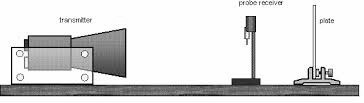
\includegraphics[width=10cm]{Microwaves.jpg}\\
The receiver can be moved to find areas of nodes or antinodes
\subsection{Harmonics}
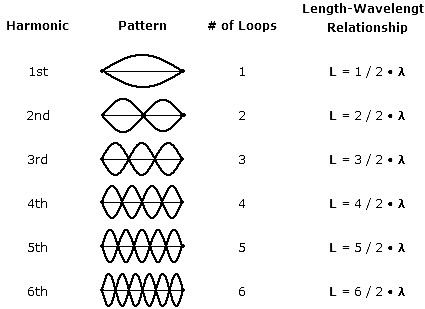
\includegraphics[width=15cm]{Harmonics.jpg}\\


\end{document}
